\documentclass[11pt, a4paper]{article}
%\usepackage{proj1}
\usepackage{natbib}
\usepackage{fancyhdr}  
\usepackage{subcaption}
\usepackage{caption}
\usepackage{graphicx}
\linespread{1.25} 
\setlength{\parindent}{0cm}
\graphicspath{{Images/}}
\usepackage{hyperref}
\usepackage{amsmath}
\usepackage{amsfonts}
\usepackage{amssymb}
\usepackage{amsthm}
\usepackage{mathtools}
\usepackage{commath}

%\usepackage[sc,osf]{mathpazo}
\usepackage{subcaption}
\usepackage[a4paper, top=1in, left=1.0in, right=1.0in, bottom=1in, includehead, includefoot]{geometry} %Usually have top as 1in

\usepackage{listings}
\usepackage{color} %red, green, blue, yellow, cyan, magenta, black, white
\definecolor{mygreen}{RGB}{28,172,0} % color values Red, Green, Blue
\definecolor{mylilas}{RGB}{170,55,241}


\hypersetup{colorlinks,linkcolor={black},citecolor={blue},urlcolor={black}}
\usepackage{color}
\urlstyle{same}


\theoremstyle{definition}
\newtheorem{definition}{Definition}[section]

\title{Exact Solutions for the Full Problem \\with Force Control and with Flow Control}
\date{}
\newcommand{\Sta}{\rho}
\newcommand{\Adj}{p}
\newcommand{\Con}{u}

\pagenumbering{gobble}
\begin{document}
	
\section*{Report 30/04/2020 (2)}

\section{Other comments on the 1D problems}
I have tried some of the problems in the other report with Picard, which works but is slower. I have also tried different $\beta$ values ($\beta = 10^{1}$ and $\beta = 10^3$) and these work as expected( $\beta = 10^{1}$ gives small improvement of $J_{FW}$, $\beta = 10^3$ solves in one iteration for the most part).\\
Looking at the first Neumann example from Report $1$ again:
Choosing $\gamma = 0.5$ and $\gamma =-0.5$ with $\beta = 10^{-1}$ shows the difference in the two $\gamma$ values, see Figure \ref{Res22}. 
\begin{figure}[h]
	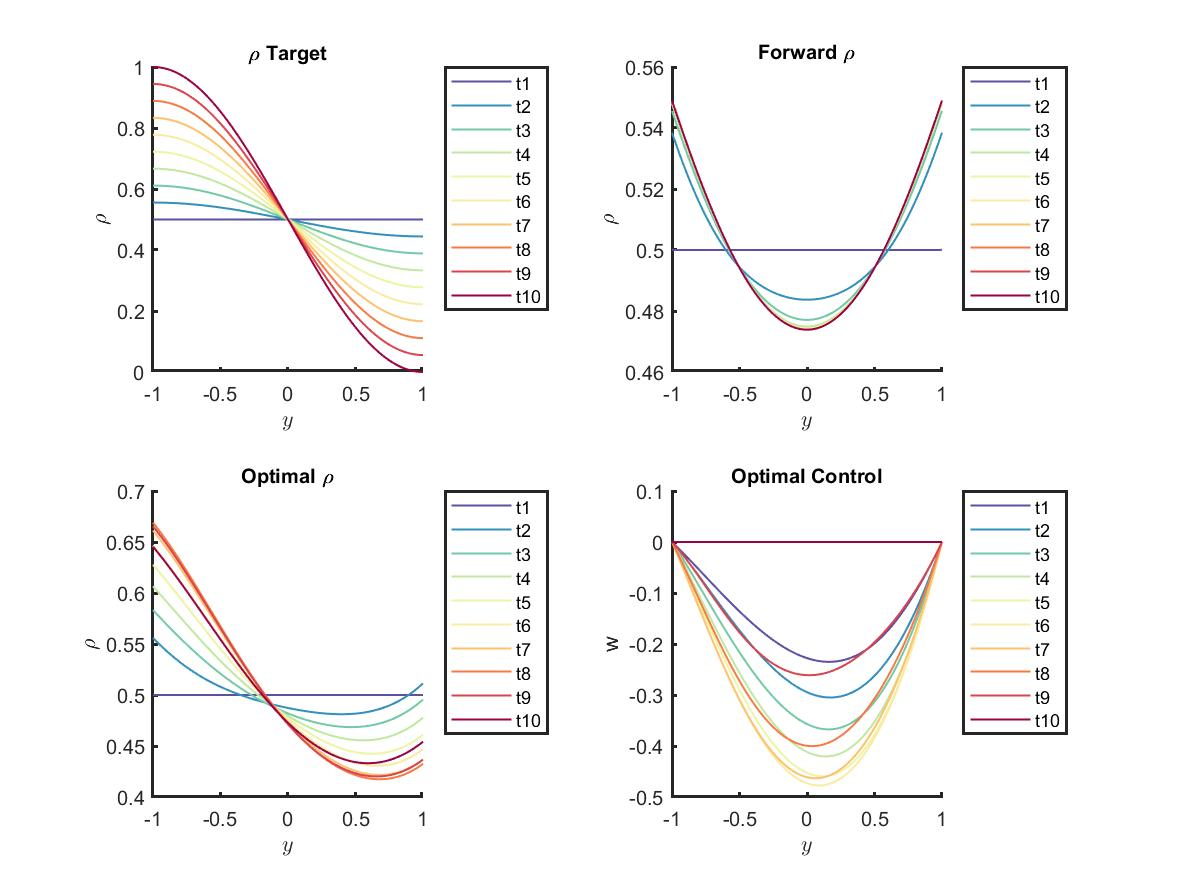
\includegraphics[scale=0.3]{Res21.jpg}
	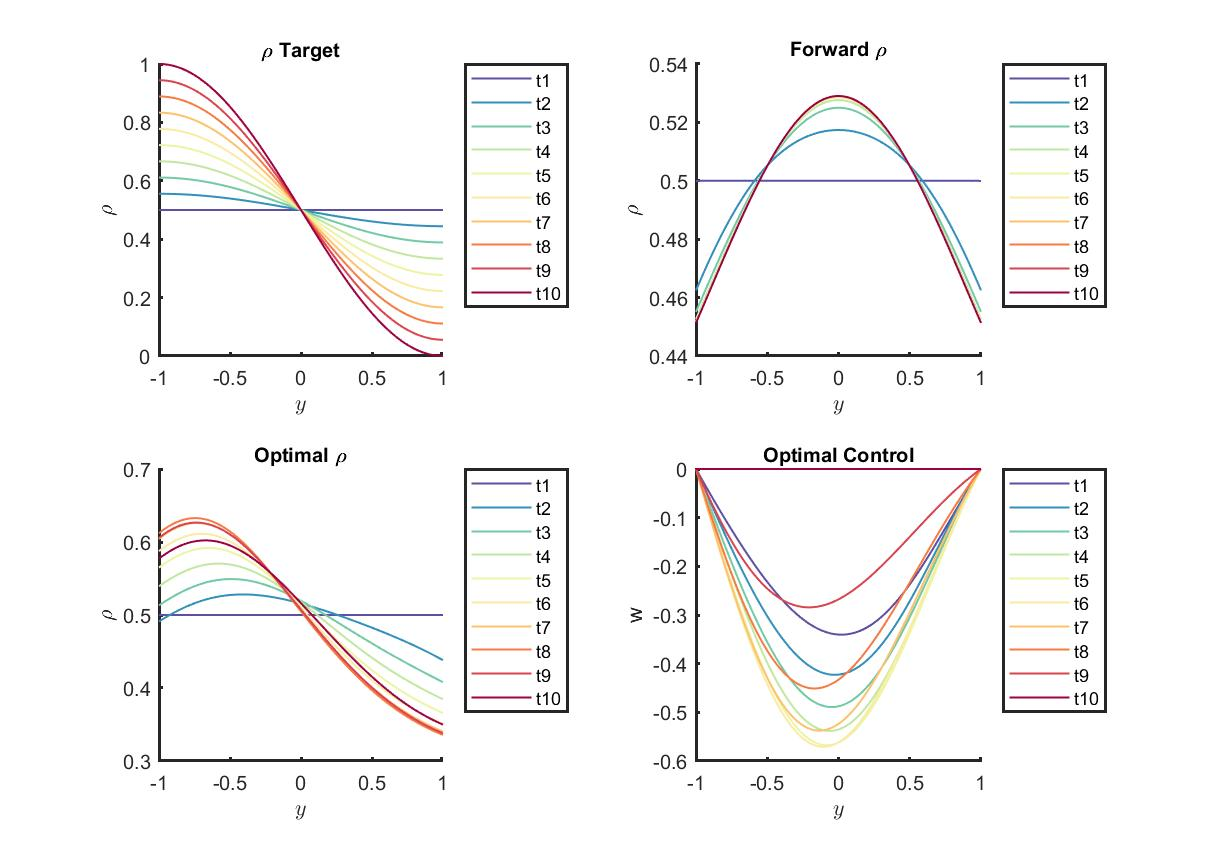
\includegraphics[scale=0.3]{Res22.jpg}
	\caption{Results for Neumann Flow, $\gamma = -0.5$ and $\gamma =0.5$.}
	\label{Res22}
\end{figure}
\section{Notes on 2D Problem}

As mentioned in the email, the 2D problem with strong interaction does not work. For $N1 \times N2 = 60$, $n=61$ and almost order $1$ interaction strength, the Forward Problem doesn't return the solution at all time points. The initial condition was $0.5$, a constant. This is for $\beta = 10^{-3}$ and $\beta = 10^{-1}$. 
For $\beta = 10^{-3}$ and interaction $\gamma = -0.5$, $\gamma = 0.5$, the forward problem is running correctly, but the optimization diverges at around $0.19$, with $\hat \rho = 0.5(1-t) + t((1/2)\sin(\pi(y1 - 2)/2) \sin(\pi(y2 - 2)/2) + 1/2)$.\\
Changing $\hat \rho$ but messing up the first term...:
\begin{align*}
\hat \rho = 0.5(1-t) + t(1-t)0.5 + t(1/4)((\cos(\pi y1 + \pi)+2)(\cos(\pi y2 + \pi)+2)).
\end{align*} 
This converges for $\gamma =0$ and $\gamma = -0.2$, but is not exactly the case I wanted to consider. $J_{FW} = 0.4635 $, $J_{Opt} = 0.2766$, see Figure \ref{Res2D1}.
\begin{figure}[h]
	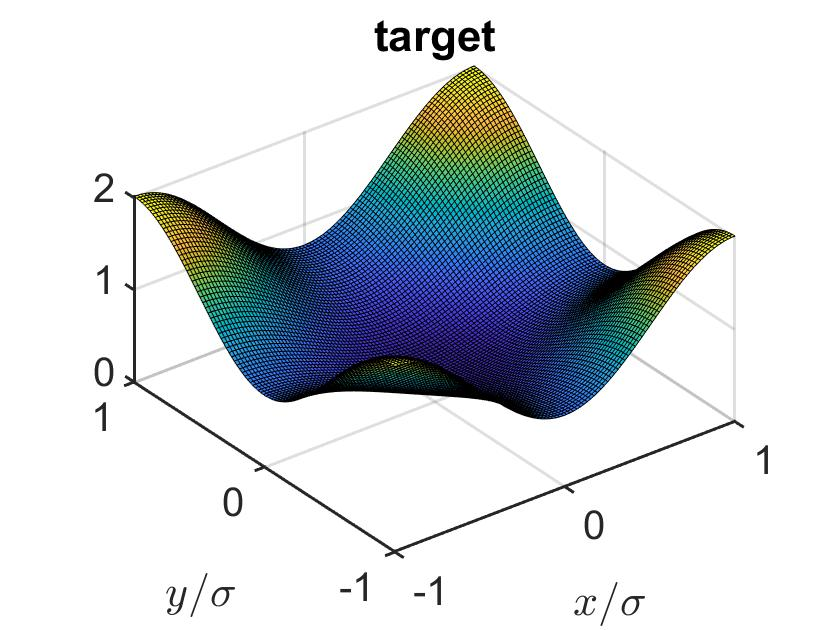
\includegraphics[scale=0.3]{Tar2D1.jpg}
	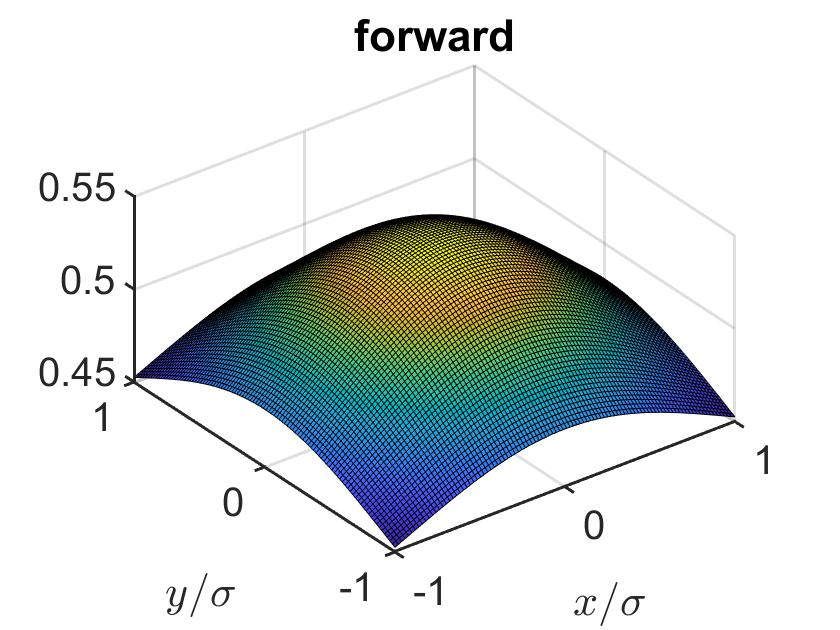
\includegraphics[scale=0.3]{FW2D1.jpg}
	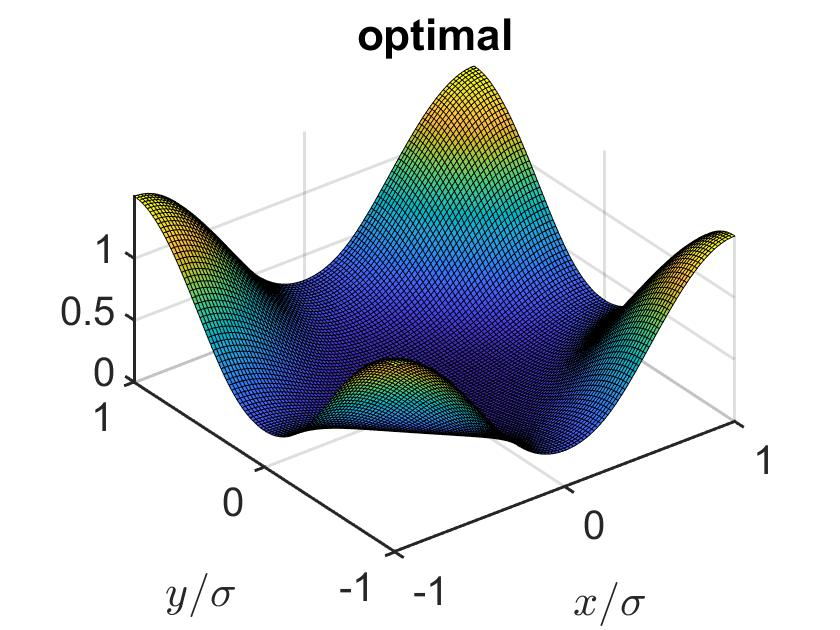
\includegraphics[scale=0.3]{Opt2D1.jpg}
	\caption{Results for Neumann Flow, $\gamma = -0.2$.}
	\label{Res2D1}
\end{figure}
\\
\\
Choosing $\rho_{IC}=0.5$ and $\gamma =-0.5$, the forward problem shows a considerable 'bump' in the middle of the domain. For $\gamma = -0.7$, this already looks very steep, so I am not surprised that larger values of $\gamma$ cause the forward problem to fail.\\
Choosing $\hat \rho$ to also be a 'bump' in the middle of the domain:
\begin{align*}
\hat \rho = 0.5(1-t) + t\frac{1}{4}((\cos(\pi y1)+2)(\cos(\pi y2)+2)).
\end{align*}
\section{Quick demo of the plotting function}
Three plots produced with the new plotting function, see Figures \ref{Demo1}, \ref{Demo2} and \ref{Demo3}.
\begin{figure}[h]
	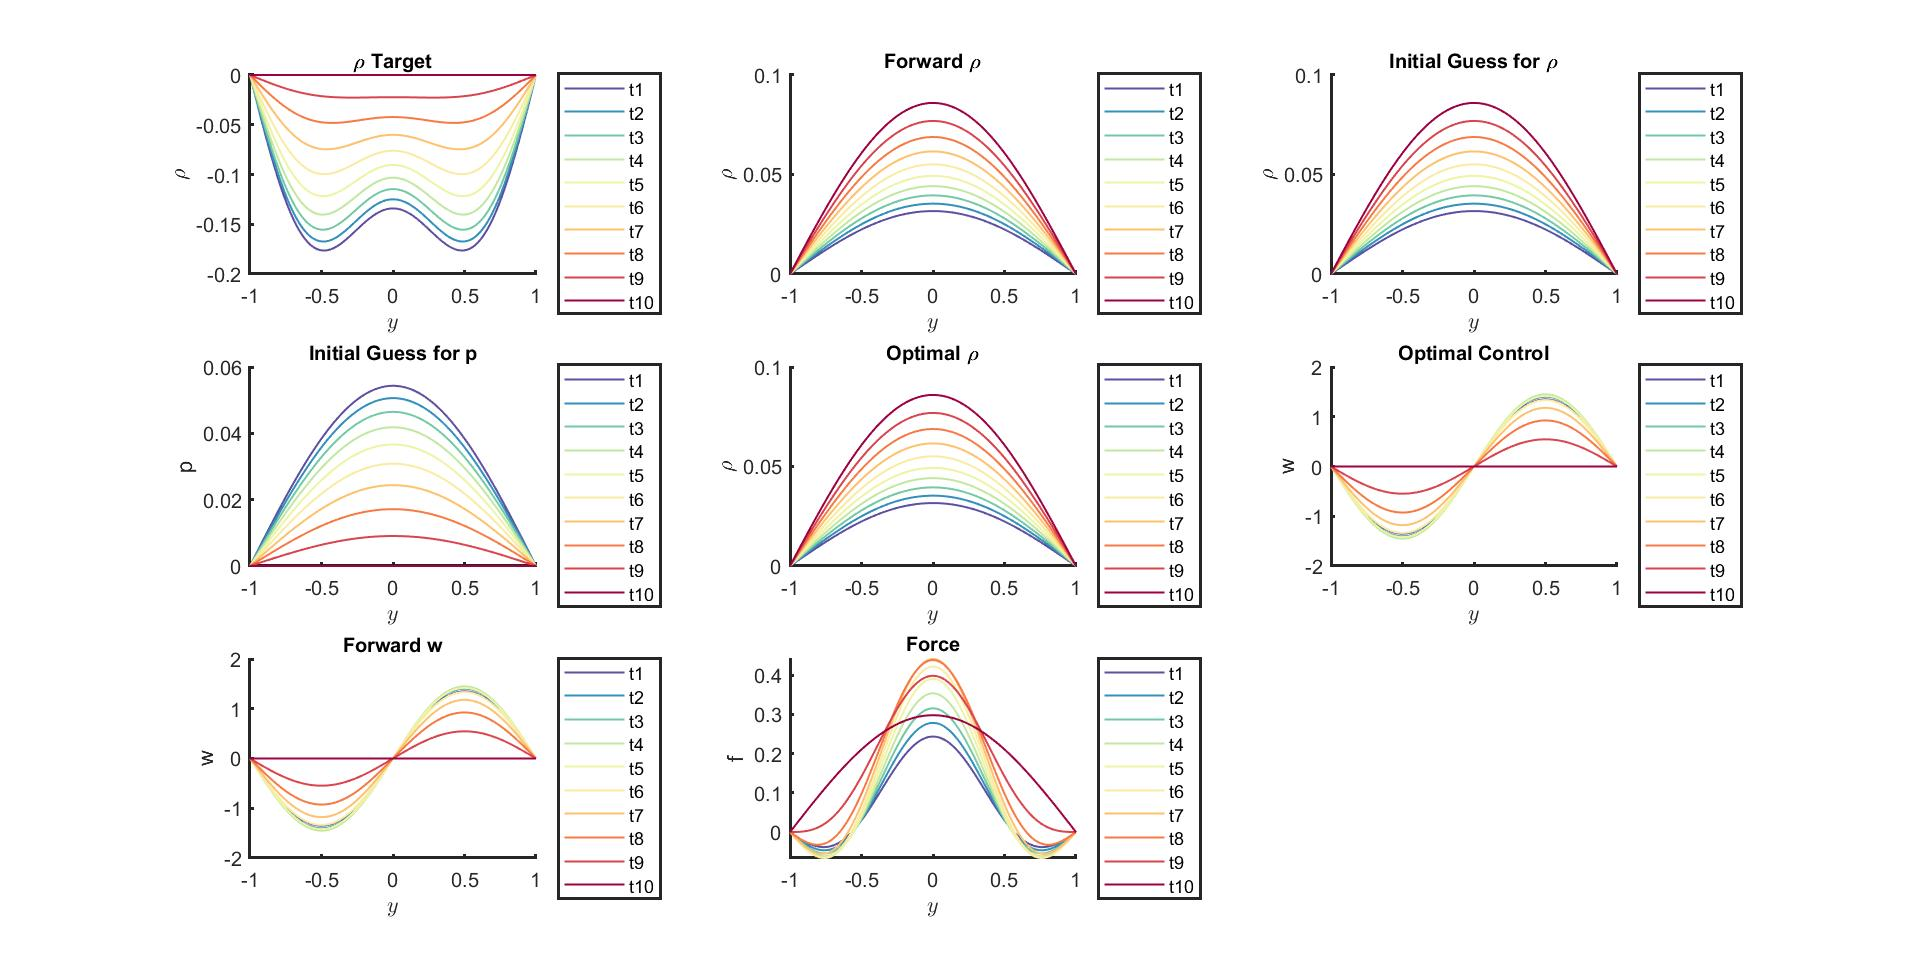
\includegraphics[scale=0.3]{Demo1.jpg}
	\caption{Demo of plotting function 1.}
	\label{Demo1}
\end{figure}
\begin{figure}[h]
	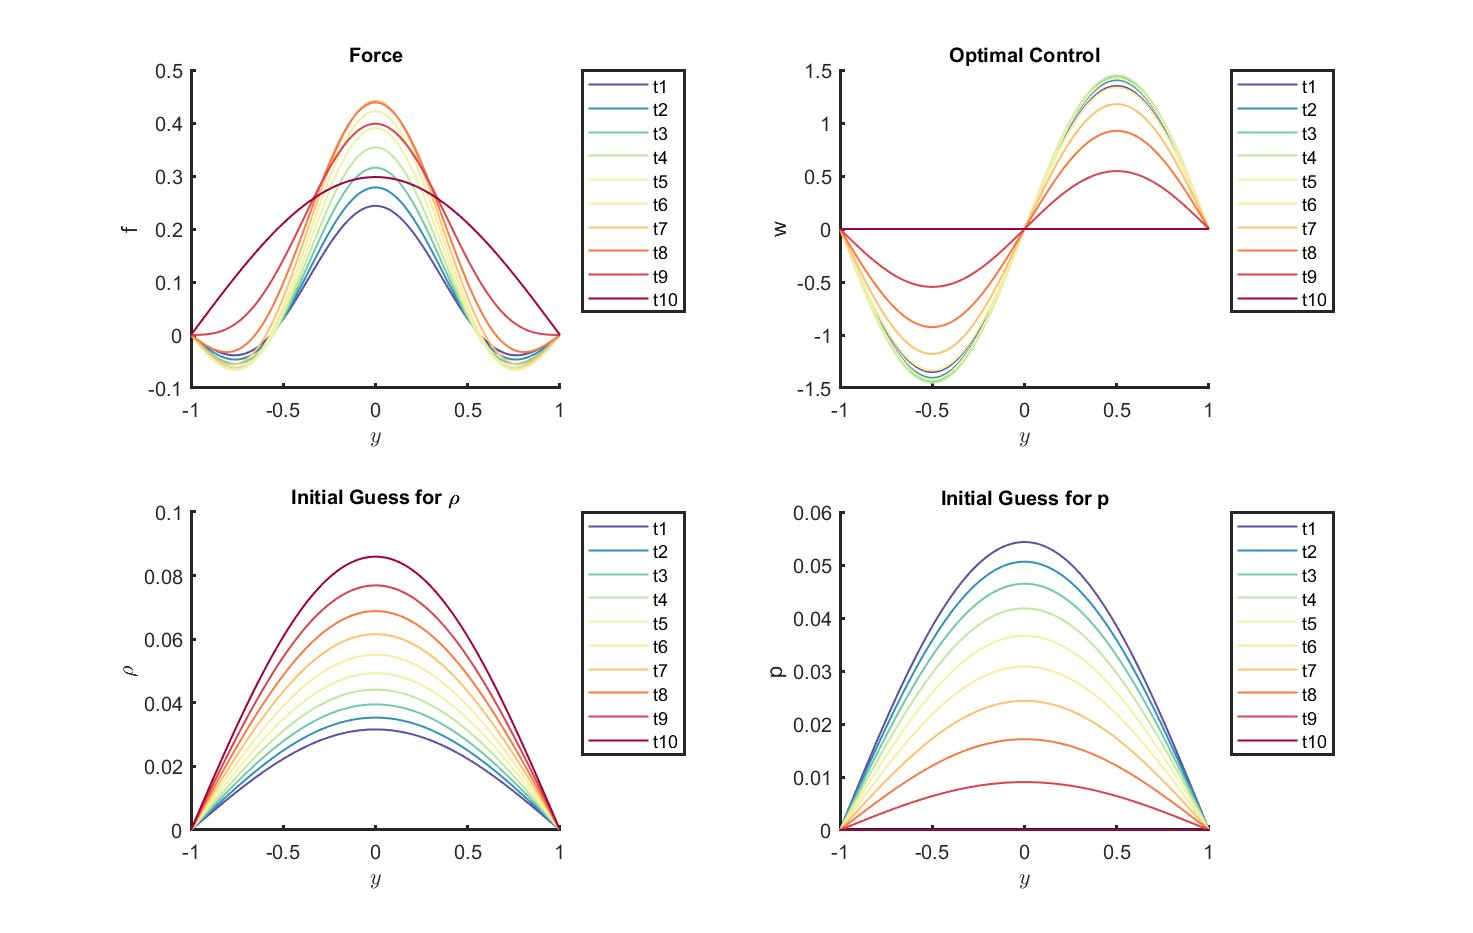
\includegraphics[scale=0.3]{Demo2.jpg}
	\caption{Demo of plotting function 2.}
	\label{Demo2}
\end{figure}
\begin{figure}[h]
	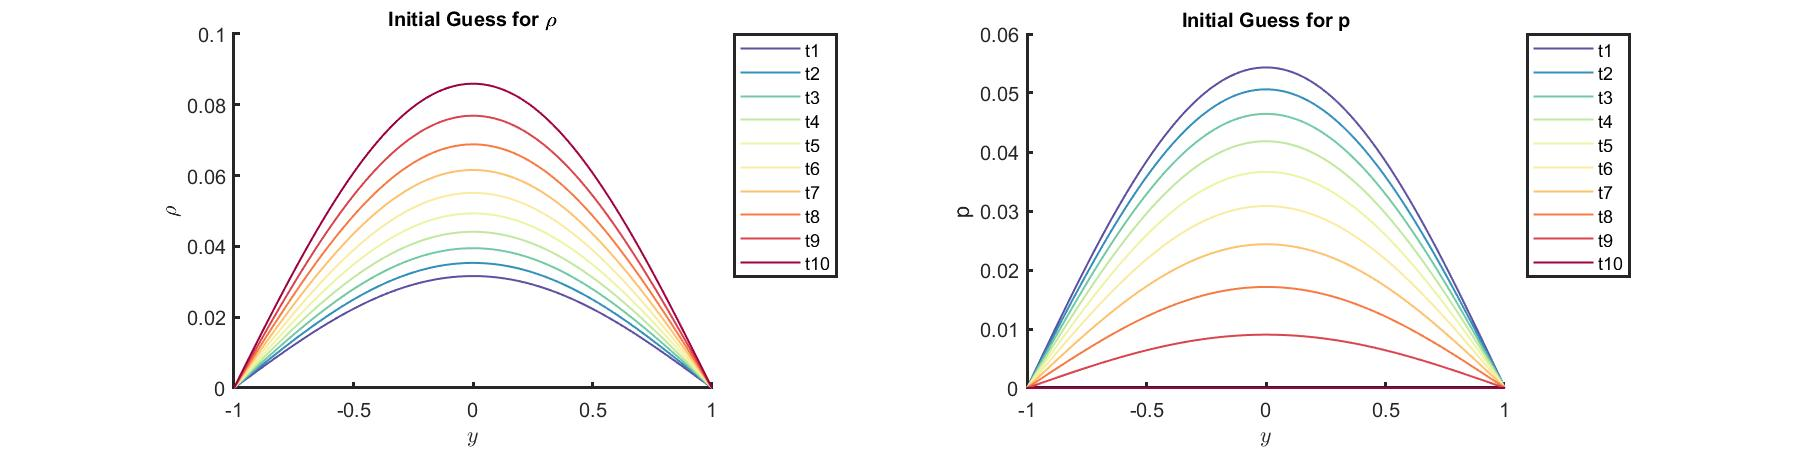
\includegraphics[scale=0.3]{Demo3.jpg}
	\caption{Demo of plotting function 3.}
	\label{Demo3}
\end{figure}
\section{Other things to discuss}

- 2D plotting function \\
\\
- Presentation at the E-symposium\\
- End of year review\\
- Class choices

\end{document}